\subsection{Методика парсинга}
Понимание сайта --- важная часть абсолютно любого парсинга данных. Как понятно из определения, необходимо собирать информацию.
Для того, чтобы собирать информацию, необходимо знать как она расположена.
Для того, чтобы понимать как расположена информация, необходимо исселодовать пути появления этой информации перед пользователем и 
выяснить откуда она берется.

Плавно мы подбираемся к тому, что знание устройства сайта, клиентской части и сервера --- необходимы для ранее сказанного парсинга данных.
Другими словами, для парсинга данных с сайта необходимо полностью понимать как тот устроен. 
Если же не получается полностью изучить, то необходимо понять, какие данные должны использоваться, чтобы в конечном итоге достичь нужного результата.
Нужно цепляться буквально за любую крупицу данных, которая может так или иначе помочь.

\subsubsection{Взаимодействие с сервером}
Для поиска подобной крупицы информации нужно понимать, что ничего не происходит из ниоткуда. Везде есть какие-то следы.
Они могут быть зашифрованы, или спрятаны за тонной других запросов. Но информация откуда-то получается.
Нужно сделать оговорку, потому что есть сайты, которые не используют сервер для получения какой-либо информации, 
а она уже сразу закодирована в верстке сайта. Такими сайтами называются <<визиткой>>.
Как понятно из навзвания, такие сайты нужны для того, чтобы красиво продемонстрировать род деятильности, прорекламировать компанию,
которую представляет тот или иной сотрудник и указать там контакты для сотрудничества.
Обычно такие сайты одностроничные, под собой не имеют никакой логики. Такие сайты очень удобно парсить.
Но чаще всего человек сталкивается с сложными сайтами со сложной логикой, где есть большая база пользователей и контета.
Такие сайты просто обязаны обращаться за какой-то логикой на сервер.

Можно заметить, что в разделе \ref{js-ref} упоминается JS --- логическая сторона сайта. Почему не пользоваться этой замечательной компонетой сайта для различной логики?
Дело, конечно же, в безопасности. Куда более надежно будет положить какую-то информацию в переменную, а потом ее в будущем отобразить на странице при помощи, например, jQuery.
Никто не хочет, чтобы алгоритмы обработки личной информации лежали перед всеми на видном месте, чтобы их можно было запустить и все расшифровать.
Или как еще по-другому можно хранить миллионы миллиардов информации?

Итак, так как предмет исследования как раз идет за нужной информацией на сервер, 
необходимо понять из каких крупиц информации создаются следующие более сложные запросы на сервер.
Для этого необходимо изучить выдаваемую информацию на сайте, запросы, которые исполняются в процессе загрузки страницы.
Исследование нужно производить с конца, идя в самое начало.
Например, если мне нужно достать нужную мне картинку, то мне нужно найти запрос, который эту картинку запрашивает.
Далее нужно найти запрос, который делает предыдущий запрос и так до самого основание.

Таким образом мы можем понять как сайт взаимодействует с сервером при различном получении разных страниц.

\subsubsection{Изучение данных}
Необходимо сделать несколько оговорок:
\begin{itemize}
    \item все примеры будут продемонстрированы в браузере Google Chrome, так как в нём имеется богатый инструментарий для программистов, а также поддерживается огромное колличество сайтов, ведь именно этот браузер является самым популярным \cite{broser-popularity-cite},
    \item комбинации клавиш, продемонстрированные в примерах, актуальны для операционной системы Windows.
\end{itemize}

Для поиска информации необходимо пользоваться инструментом разработчика. Открывается данное меню разработчика при помощи нажатия клавиши F12. 
На рисунке~\ref{chrome-tools-pic} продемонстрировано меню.

\begin{figure}
    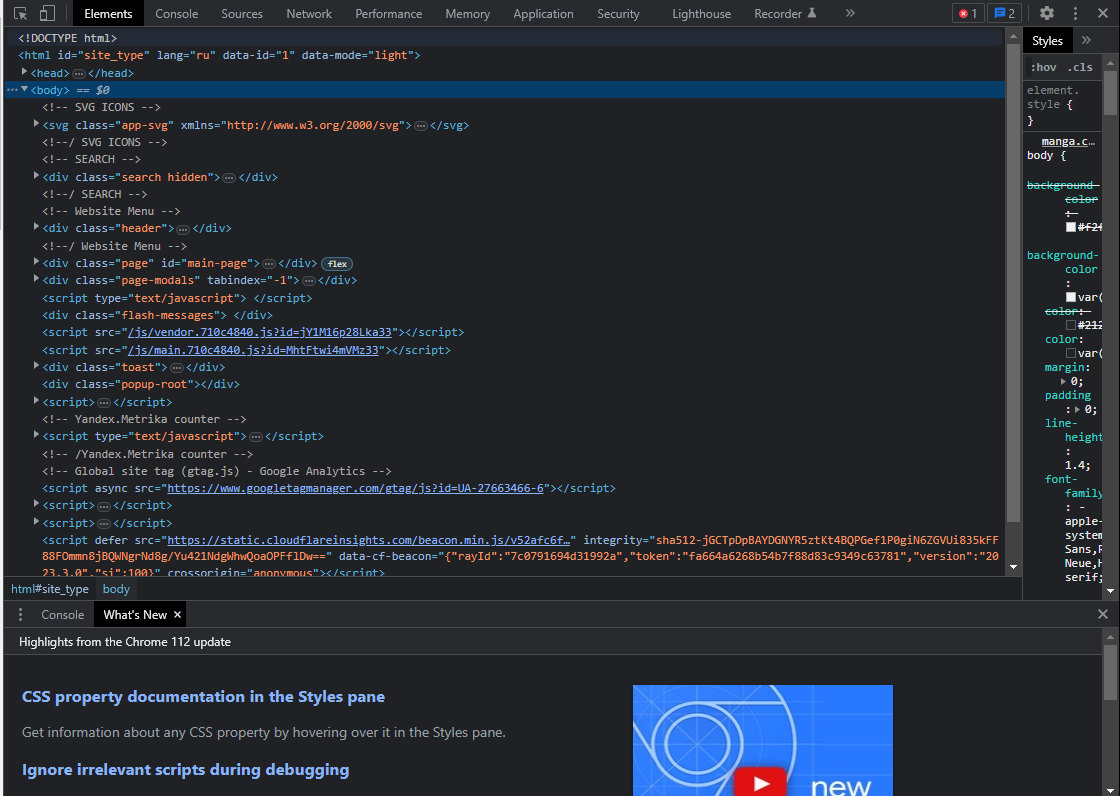
\includegraphics[scale=0.5]{imgs/chrome-tools}
    \caption{Меню разработчика}
    \label{chrome-tools-pic}
\end{figure}

У браузера есть свойство, при котором он исполняет все скрипты в тегах языка HTML. 
Как говорилось ранее, эти скрипты могут содержать запросы на сервер за получением информации на страницу.
Также еще нужно знать, что вписывание ссылки в браузер и последующем нажиманием подтверждения ввода, по сути своей делает GET запрос на домен с соответствующим роутингом.
Зная также тот факт, что на один запрос приходится один ответ, мы можем определенно точно сказать, что программа наша получит сайт с первичной информацией. 
То есть будет загружены скрипты, которые делают последующие запросы на сервер.
Из этого мы можем сделать вывод, что просто так никакая информация из ниоткуда не берется и с большой вероятностью мы при помощи только одного запроса не получим весь сайт. 
Для тестирования запросов можно пользоваться удобным инструментом postman \cite{postman-cite}.
На рисунке~\ref{postman-first-get} продемонстрирован пример одного GET запроса на сайт через инструмент postman. 
На рисунке~\ref{html-add} приложения изображена команда, которую можно сделать, чтобы посмотреть полностью код HTML.

\begin{figure}
    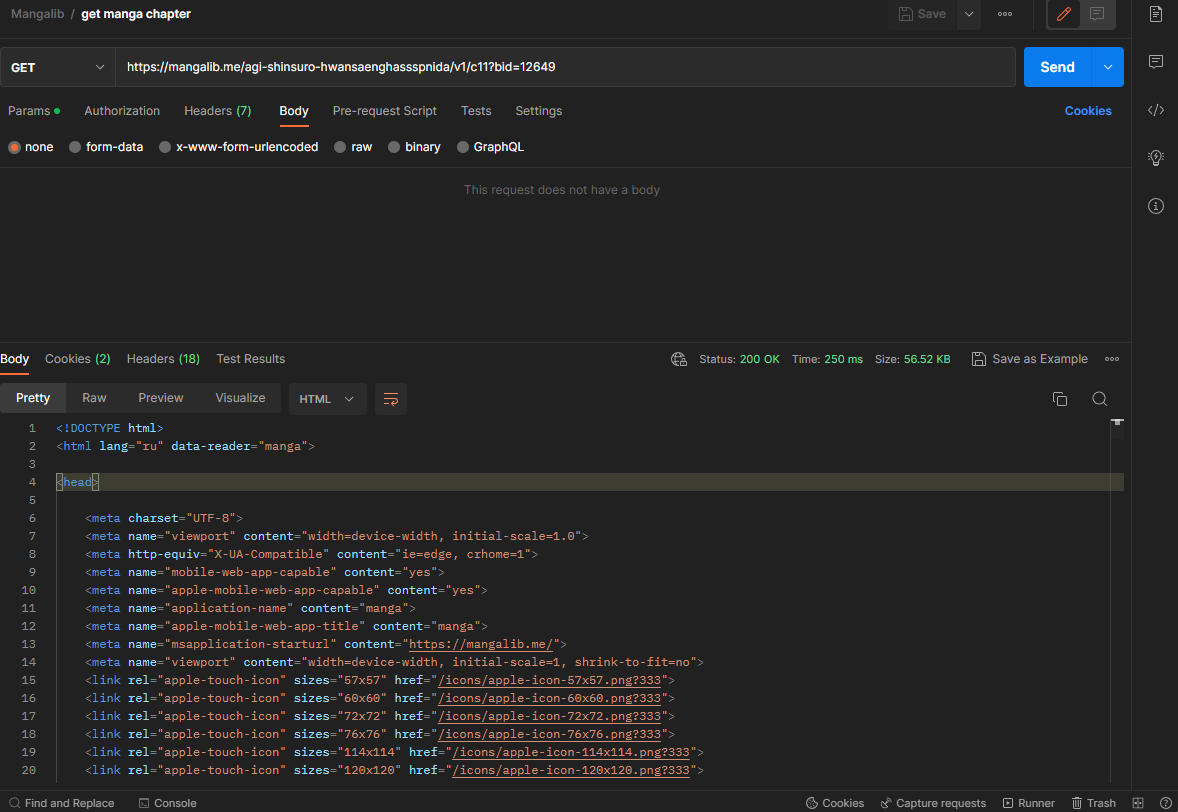
\includegraphics[scale=0.5]{imgs/postman-get-site}
    \caption{GET запрос }
    \label{postman-first-get}
\end{figure}

Из кода можно увидеть, что HTML код очень сильно отличается от того, что изображен в меню разработчика.
Это все потому, что мы не проделали все те запросы, что делает браузер, когда начинает прогрузку страницы.
К счастью, нам этого делать не надо. Это лишь доказательство того, что до любой информации мы можем одним или несколькими путями добраться.

Для того, чтобы начать изучение данных, необходимо зайти на сайт и найти самостоятельно ту конечную информацию, которая нужна. 
В данном случае ведется поиск картинок.
После того, как мы нашли нужную картинку, необходимо понять как выглядит ссылка на нее.
Исходя из той логики, что разработчик сайта будет составлять ссылку из абсолютно случайного набора букв и цифр -- крайне мала, так как это решение бесполезно и очень сильно влияет на быстроту разботки в худшую сторону,
мы можем попробовать догадаться по какой логике конструируется ссылка на ресурс. Итак, чтобы посмотреть на ссылку картини, нам необходимо посмотреть код этой картинки в HTML.
На рисунке~\ref{chrome-tools-image-tag-pic} видно, как выделен тэг картинки, которую мы бы хотели получить. 

\begin{figure}
    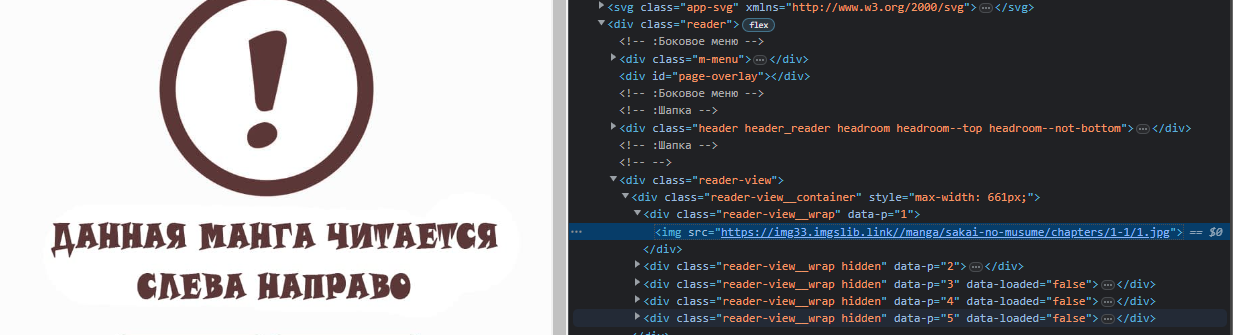
\includegraphics[scale=0.5]{imgs/chrome-tools-image-tag}
    \caption{Представление картинки в кода HTML}
    \label{chrome-tools-image-tag-pic}
\end{figure}

Посмотрев так на другие картинки, можно увидеть, что у них у всех есть один источник.
А ссылка формируется по паттерну из рисунка~\ref{image-pattern-add}. Следовательно возможно эту ссылку конфигурировать своими руками в сервисе.
Для этого нам нужны:

\begin{itemize}
    \item название манги,
    \item правильных id главы,
    \item хеш картинки.
\end{itemize}

Теперь необходимо узнать где на странице еще лежит вышеописанная информация. Для этого нам нужно проанализировать запросы.
Для этого нам пригодится вкладка Network в меню разработчика.
На странице картинки открываем меню разработчика и перезагружаем страницу.
Это нужно для того, чтобы во вкладке появились все абсолютно запросы, которые делает браузер для того, чтобы прогрузить полностью страницу.
На рисунке~\ref{chrome-tools-network} продемонстрирован весь список запросов, который делается при загрузке страницы определенного сайта.
Очевидно этот список может отличаться от того, что продемонстрировано на рисунке~\ref{chrome-tools-network}.

\begin{figure}
    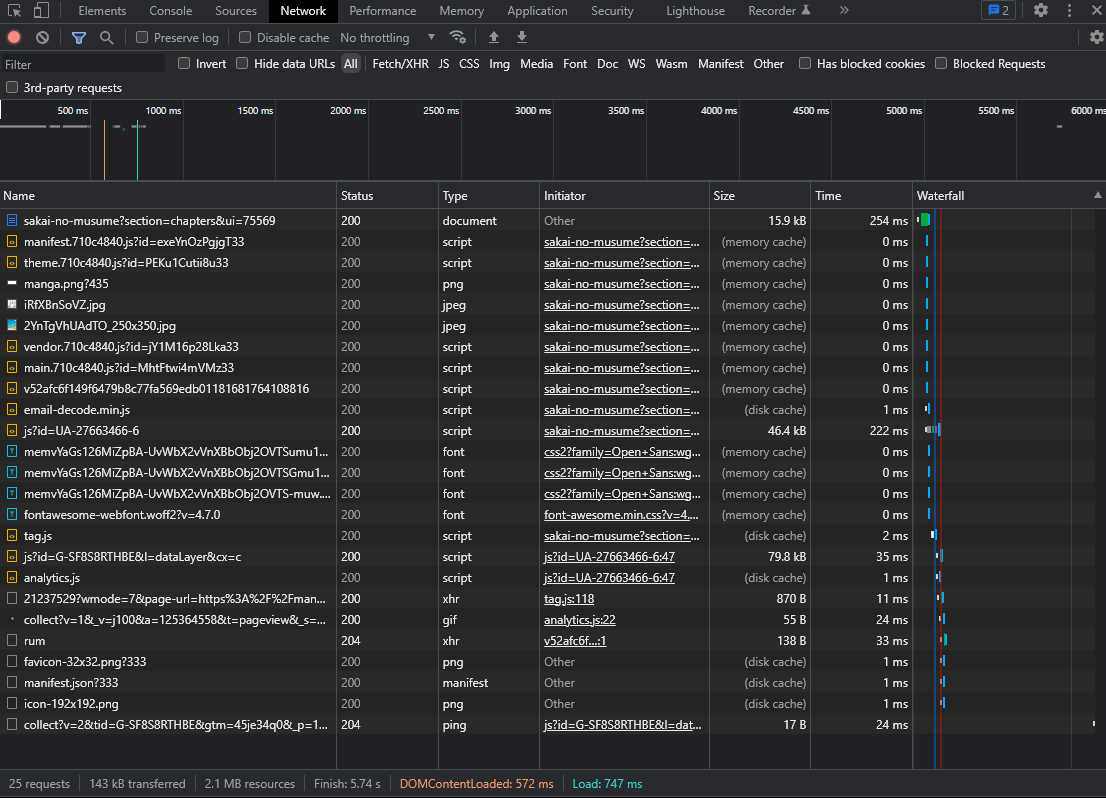
\includegraphics[scale=0.5]{imgs/network-example}
    \caption{Меню разработчика network вкладка}
    \label{chrome-tools-network}
\end{figure}

Далее необходимо найти эту картинку в запросах. В меню есть фильтр по типам файлов. Выбираем там картинки.
На рисунке~\ref{chrome-tools-network-pics} мы видим, что не очень много запросов было на картинки.
С легкостью можем найти наш файлик (на рисунке выделен).
Можно еще также заметить, что разработчики постарались и заренее прогружают следующую страницу, чтобы было проще смотреть контент.

\begin{figure}
    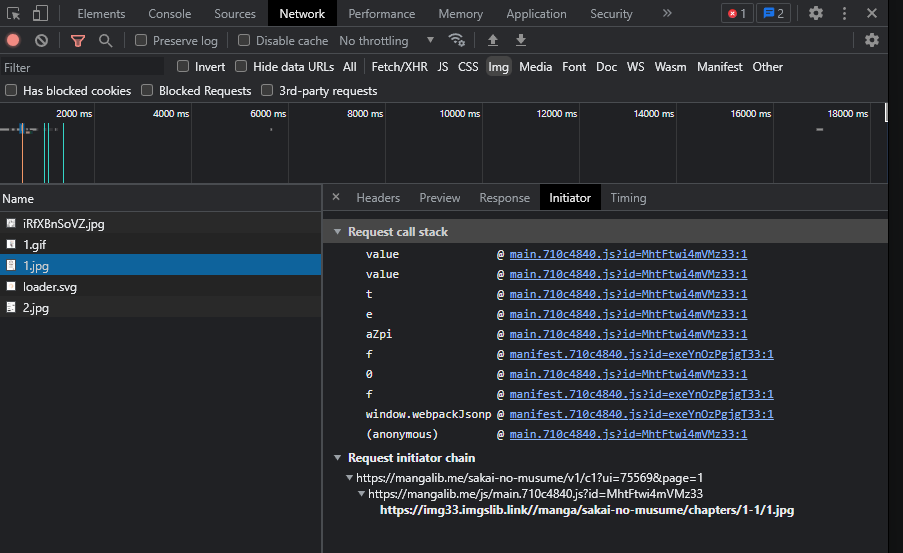
\includegraphics[scale=0.5]{imgs/network-pics}
    \caption{Меню разработчика network вкладка с фильтром по картинкам}
    \label{chrome-tools-network-pics}
\end{figure}


Теперь нам необходимо узнать как был получен запрос на эту картинку. 
Помним, что из-за особенности устройства браузера информация не появляется из ниоткуда.
Следовательно мы можем с легкостью узнать откуда пришел запрос.
Благо нам не нужно особо много, чтобы раздобыть подобного рода информацию.
Меню разработчика предоставляет интерфейс для показа стека вызова. На рисунке~\ref{chrome-tools-network-pics} можно увидеть вкладку Initiator.
Это и есть наш стэк вызовов.

На самом деле, если мы будем смотреть код каждого запроса, сможем легко закопаться в нем, так как чаще всего подобного рода сайты подключают разные сервисы для генерации логики.
Этот сайт не исключение. Здесь добавлена защита от DDOS атак от компании Яндекс, также трекер использования сайта.
Через подобного рода скрипты происходит процесс анализа запросов. Поэтому в середине запроса может быть сгенерированный код, который почти невозможно понять без нескольких дней его анализа.
Благо в нашем случае его анализировать не надо.
Можно начать смотреть код, который находится вокруг места, откуда произошел вызов того или иного запроса.
Таким образом натыкаемся на самый первый вызов в стеке и замечаем, что это наш любимый HTML код.
Изучив его, можно увидеть, что есть большой скрипт. В нем есть переменная <<window.\_\_DATA\_\_>> (при помощи вызова скрипта на рисунке~\ref{html-add} можно увидеть этот скриат).
Кажется это то, что нам нужно.

Переменная <<window.\_\_DATA\_\_>> --- JSON, в котором явно написана информация о манге.
Исследовав этот объект, обнаруживаем, что там есть информация о названиях каждой страницы. Можно также ваявить и сколько страниц в данной конкретной главе.
На рисунке~\ref{json-structs-parsing} можно посмотреть на получившуюся структуру, в которую можно парсить из JSON.

\begin{figure}
	\begin{lstlisting}[language=go]
		type pageList struct {
            Page int    `json:"p"`
            Url  string `json:"u"`
        }
	\end{lstlisting}
	\caption{Структры содержания информации о главах и картинках}
	\label{json-structs-parsing}
\end{figure}

В Url атрибуте хранится тот самый хэш картинки.
ID главы можно узнать из атрибутов на той же странице.
Название манги совсем просто найти. Оно находится буквально в каждой ссылке данного сайта. Поэтому можно просто скопировать название оттуда.

Примеры выше были для сайта mangalib.me, участвующий в итоговом дипломе.
Анализ каждого сайта происходит в индивидуальном порядке, так как везде свои разные алгоритмы и подходы.
Задача микросервиса сделать так, чтобы добавление новых сайтов было достаточно простым и требовало исключительно анализа и исполнении всех алгоритмов для автоматического поиска.


\subsubsection{Сайты с API}
Есть некоторые сайты, разработчики которых подумали о пользователях и о том, что эти пользователи возможно хотели бы автоматизировать процесс поиска и скачивания контента.
Одним из таких сайтов является mangadex \cite{mangadex-cite}.

Для подобных сайтов нет необходимости заниматься реверс-инженерингом, как было представлено выше. 
Достаточно изучить документацию \cite{mangadex-api-cite} и найти хендлеры, которые выполняют поставленную задачу и использовать их.
Однако, это не означает, что предварительную обработку не нужно делать.
Благо вышесказанный сайт имеет много примеров использования и свой SWAGGER \cite{swagger-cite} для тестирования.

Тестирование подобного API происходит через принцип <<проб и ошибок>>, так как не всегда случается такое, что появляется на выходе ожидаемая информация.
В некоторых случаях нужно заниматься ее обработкой.